\chapter{项目背景}
  LED产业发展迅速,在时装、新媒体艺术、纺织等领域,LED因其体积小、可靠性高、能耗低的特点,收到青睐,特别是柔性LED相关技术,更是亟待发展。
  
\chapter{研究计划}
目前将进行柔性电路的研究和测试,之后将分为以下几个应用场景进行开发:(不限于以下提出的应用场景)

{\heiti 应用场景1:脑电控制的交互式RGB-LED点阵穿戴式设备 }

通过检测脑电信号,将使用者的心情以Emoji等形式在休闲帽等穿戴式设备上用柔性LED阵列显示,从而达到交互的目的。

同时,穿戴式设备上的图案可以自定义,作为一种现代化的自我表达形式。还可以借助其他模块实现类似的附加功能,如:心率+呼吸+体温检测等。

由于柔性电路耐水洗且可靠,可以直接使用洗衣机清洗,做到了无负担的使用体验。相对于其他嵌入式的穿戴设备优势明显,消费者认同感较高。

相关技术:

TGAM脑电模块模块可以处理并输出脑波频率谱,脑电信号质量,原始脑电波和三个Neurosky的eSense参数:专注度,放松度和眨眼侦测。由于能耗小且和人体的界面只需一个简单的干接触点,所以可以适合运用于柔性穿戴式设备中。

{\heiti 应用场景2:用于摄影行业的柔性LED平板 }

目前,摄影界普遍应用的摄影垫,制作工艺往往是LED灯带平铺在柔性材料上面,可靠性和成本低廉不可兼得,且色调单一。若应用柔性LED制作照明平板,不仅可靠性大大提升,而且柔性LED良好的性能可以实现更多的应用,如制作高尼特的球形光源等。

另外,对于个人用户的diy摄影创作,单一色源以及照射方式的摄影补光难以满足需求。柔性led照明设施能够很好地达到一种补光光源个性化定制的的效果

\chapter{类似产品分析}  
\section{The Embroidered Computer——刺绣计算机}
刺绣计算机是Irene Posch探索使用历史金刺绣材料和知识来制作可编程8位计算机。

http://www.ireneposch.net/

该产品仅由各种金属线,磁性,玻璃和金属珠子构成,并受到传统制作程序和图案的启发,对我们周围的当前数字和电子技术的外观以及我们与它们的互动提出质疑。

从技术上讲,该产品由(纺织)继电器组成,类似于半导体发明之前的早期计算机。在视觉上,金材料,这里用于它们的导电性能,排列成特定的图案以实现电子功能,主导着工作。传统上纯粹是装饰性的,这里的图案定义了它们的功能。它们裸露的核心数字例程通常隐藏在黑盒子里。邀请用户与编织纺织品的部分进行交互以为其计算。

%\begin{figure}
%\begin{minipage}{0.48\textwidth}
%  \centering
%  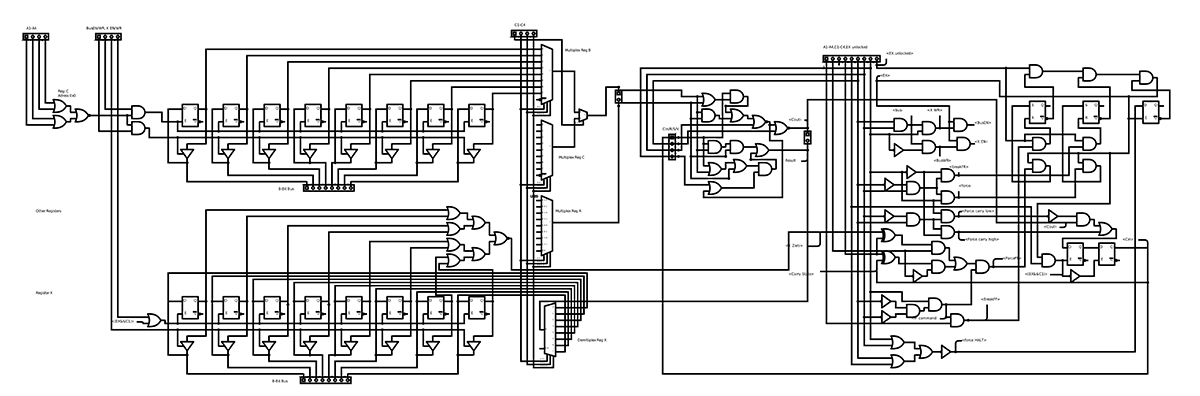
\includegraphics[height=4cm]{logic-diagram-controll-unit-1_small.jpg}
%  \caption{逻辑电路图}
%  \label{cube}
%\end{minipage}\hfill
%\begin{minipage}{0.48\textwidth}
%  \centering
%  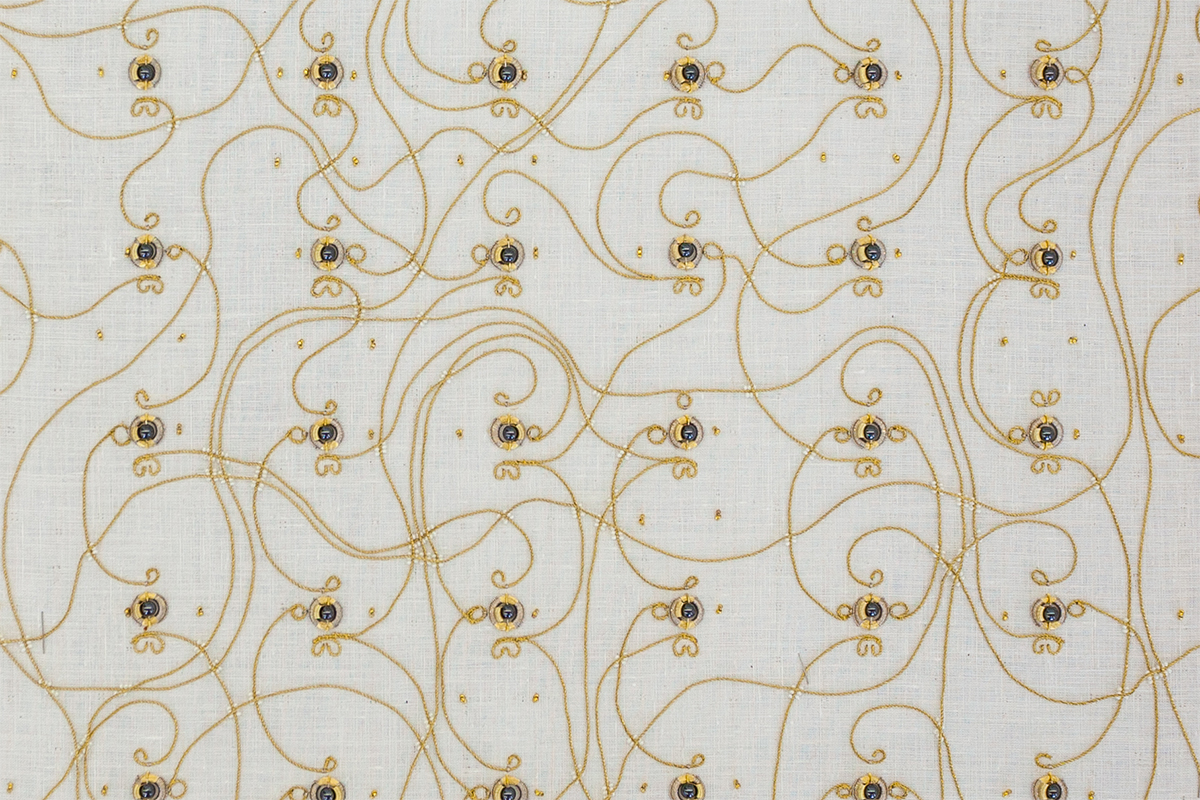
\includegraphics[height=4cm]{MG_0411_size_detail_web.jpg}
%  \caption{刺绣计算机}
%  \label{tri}
%\end{minipage}
%\end{figure}

\begin{figure}[htbp]
\centering
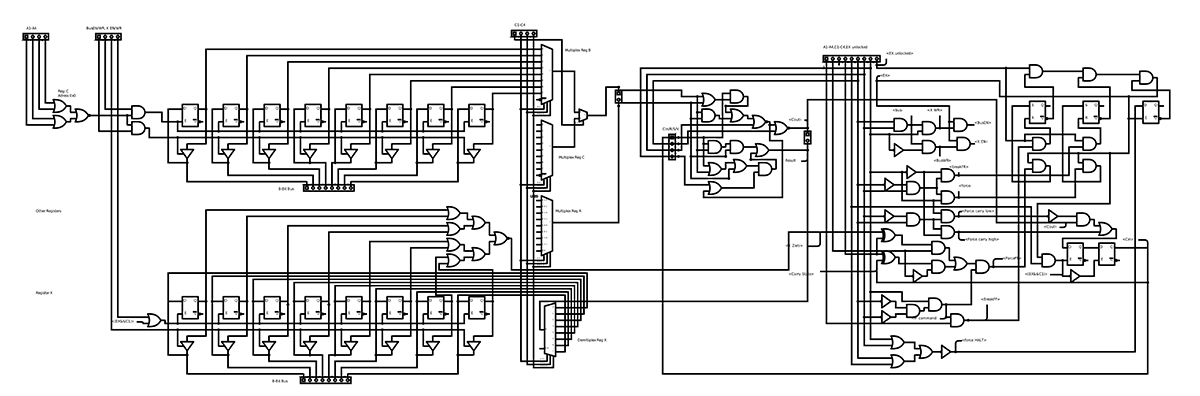
\includegraphics[width=10cm]{logic-diagram-controll-unit-1_small.jpg}
\caption{逻辑电路图} 
\label{1}
\end{figure}

\begin{figure}[htbp]
\centering
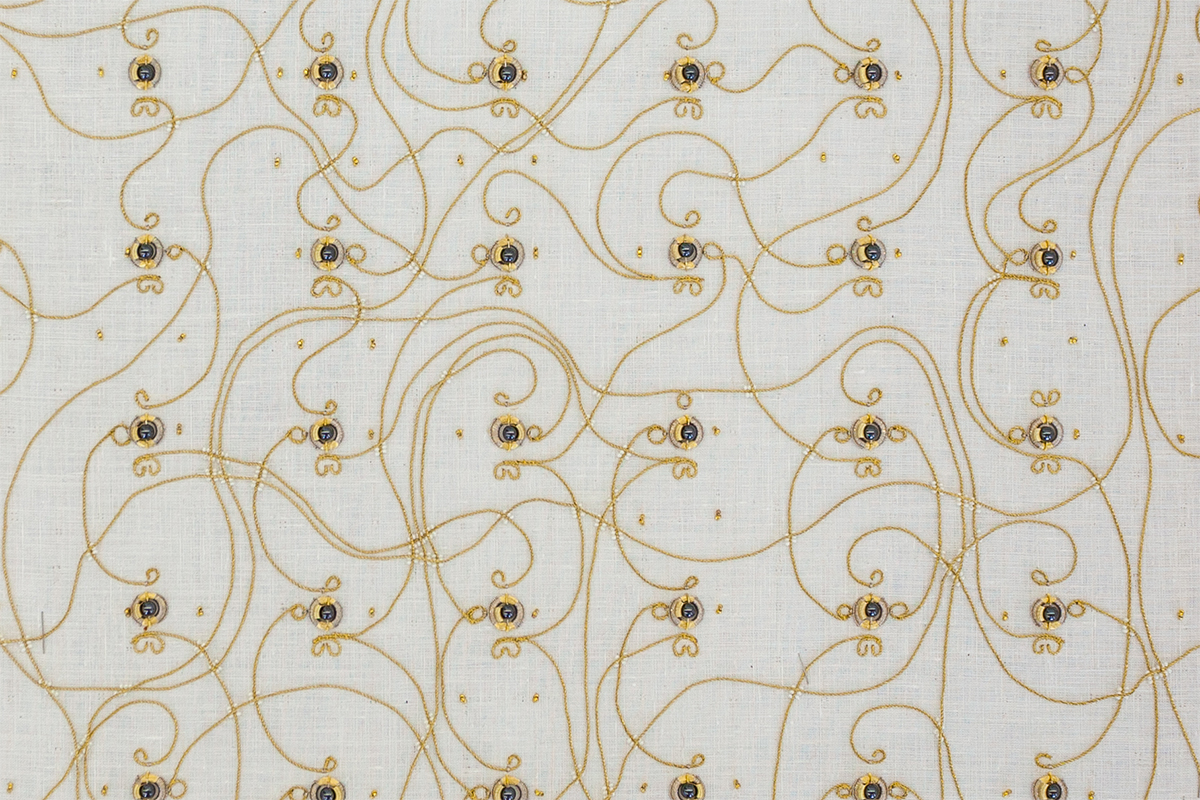
\includegraphics[width=10cm]{MG_0411_size_detail_web.jpg}
\caption{刺绣计算机} 
\label{2}
\end{figure}


由于其基本元件(门)均为继电器形式,固只能作为展品展示,无法抗冲击,但其电气链接可以供我们参考。

\newpage

\section{PIX}
PIX是一款嵌入半柔性LED面板的背包。

Pix Backpack的设计旨在让日常生活更加美好。 它结合了方便的都市背包和灵活的可编程屏幕。通过免费的IOS / Android应用程序控制Pix。 你可以在app里找到各种各样的图片/动画/小工具和游戏。只需选择你喜欢的内容,一键上传到Pix背包。

作为一款个性化背包,其设计非常个性化。但是PIX采用的不是真正柔性的LED,而是在栅格状的泡沫中嵌入LED灯,他的发光平面不能折叠且较为厚重,但在书包这一应用场景中不是一个很大的问题。

https://www.pix.style/

\begin{figure}[htbp]
\centering
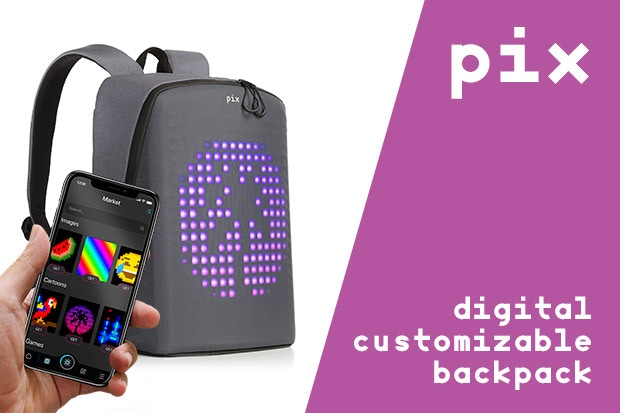
\includegraphics[width=10cm]{pix.jpg}
\caption{PIX} 
\label{p1}
\end{figure}

\section{e-broidery}

e-broidery照明纺织品保证了日夜的迷人印象。集成电子设备可实现暗淡功能和动画。 LED纺织品可以洗涤和悬垂。此外,还保留了基础面料的悬挂特性和质地 - 无论是薄纱还是厚重的织物。

除了标准产品之外,照明纺织品可以由预定的织物和刺绣选择构成。还提供基于个人客户请求的定制。包括:预选面料、刺绣、设计和灯光图案以及亮度水平等。

可以说e-broidery很好的实现了单色LED灯在织物上的嵌入,但是e-broidery并没有加入较复杂的控制(比如只有灯的闪烁控制而没有RGB控制),而且织物中只有单一型号的LED。另外e-broidery的价格十分昂贵,大约2000欧元/平方米,所以目前只有高端时装界和摄影界在使用。


\begin{figure}[htbp]
\centering
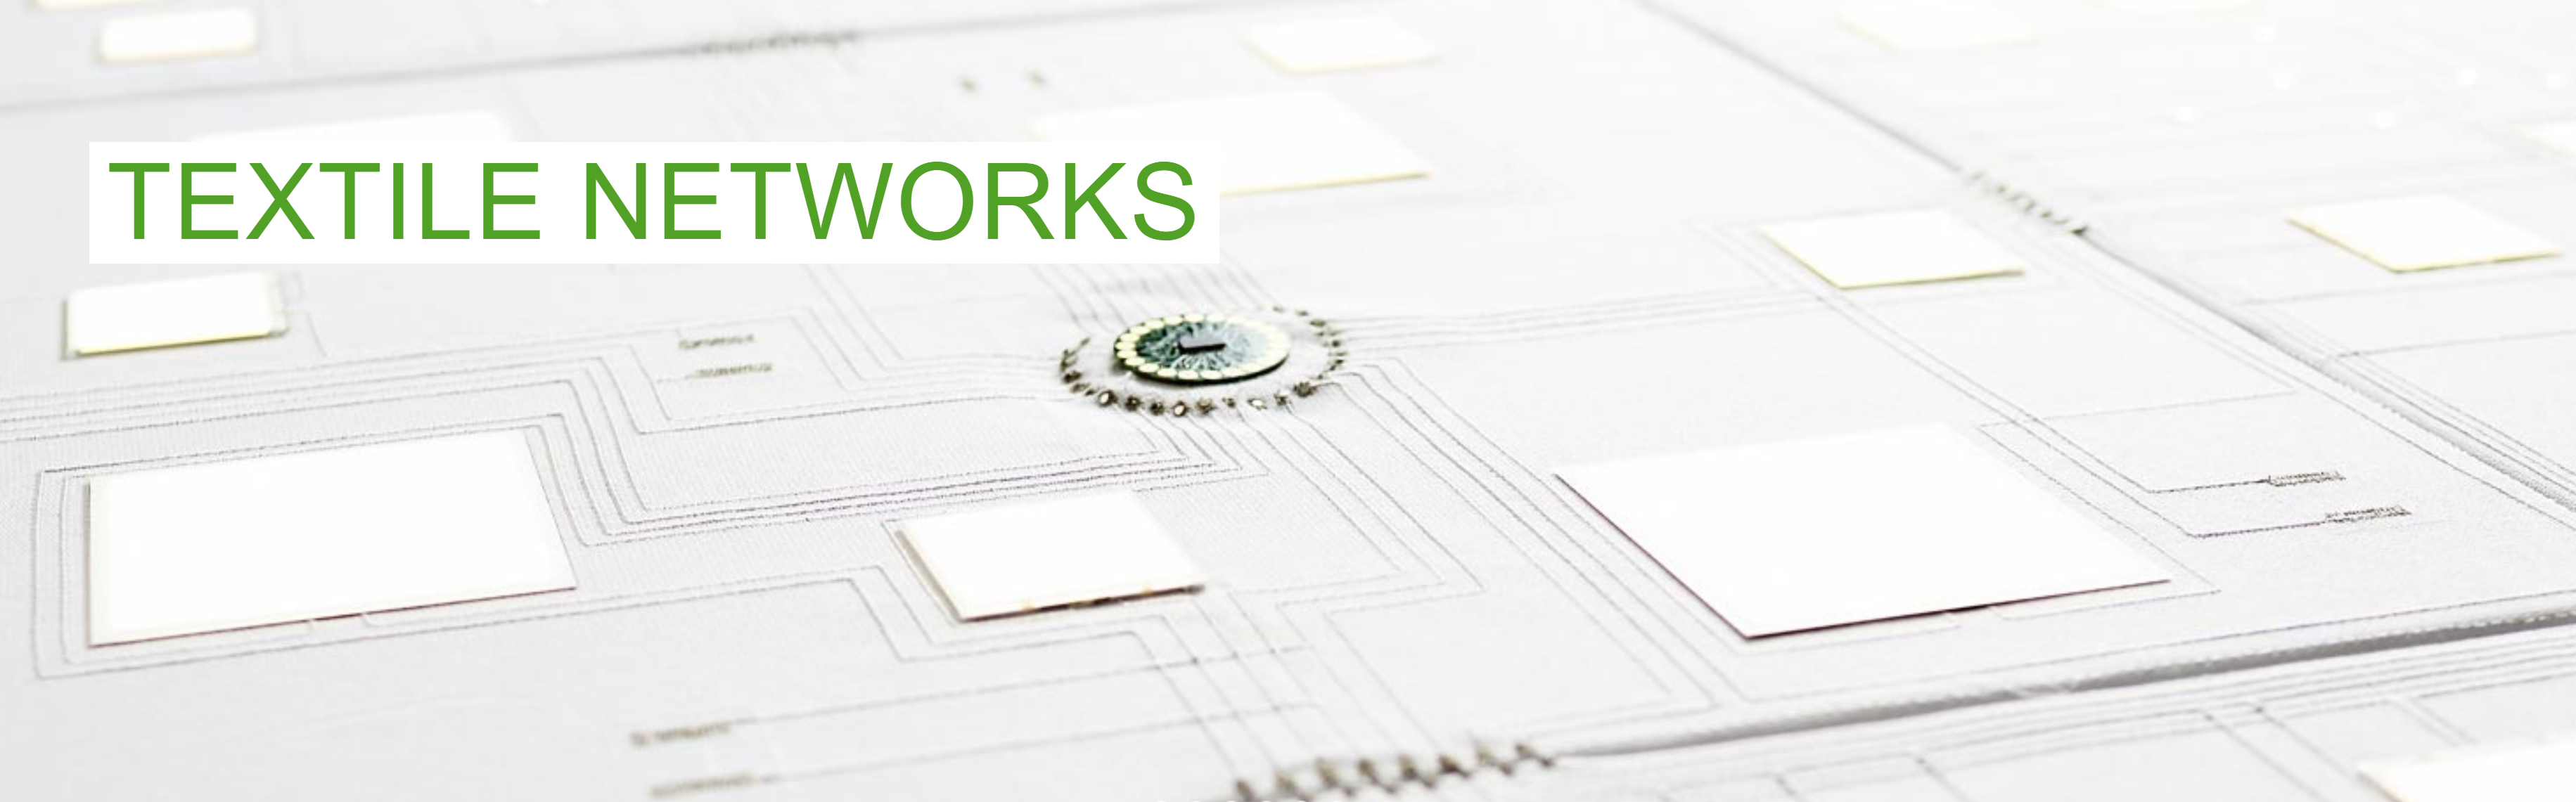
\includegraphics[width=10cm]{textile.png}
\caption{e-broidery效果图} 
\label{e1}
\end{figure}

\begin{figure}[htbp]
\centering
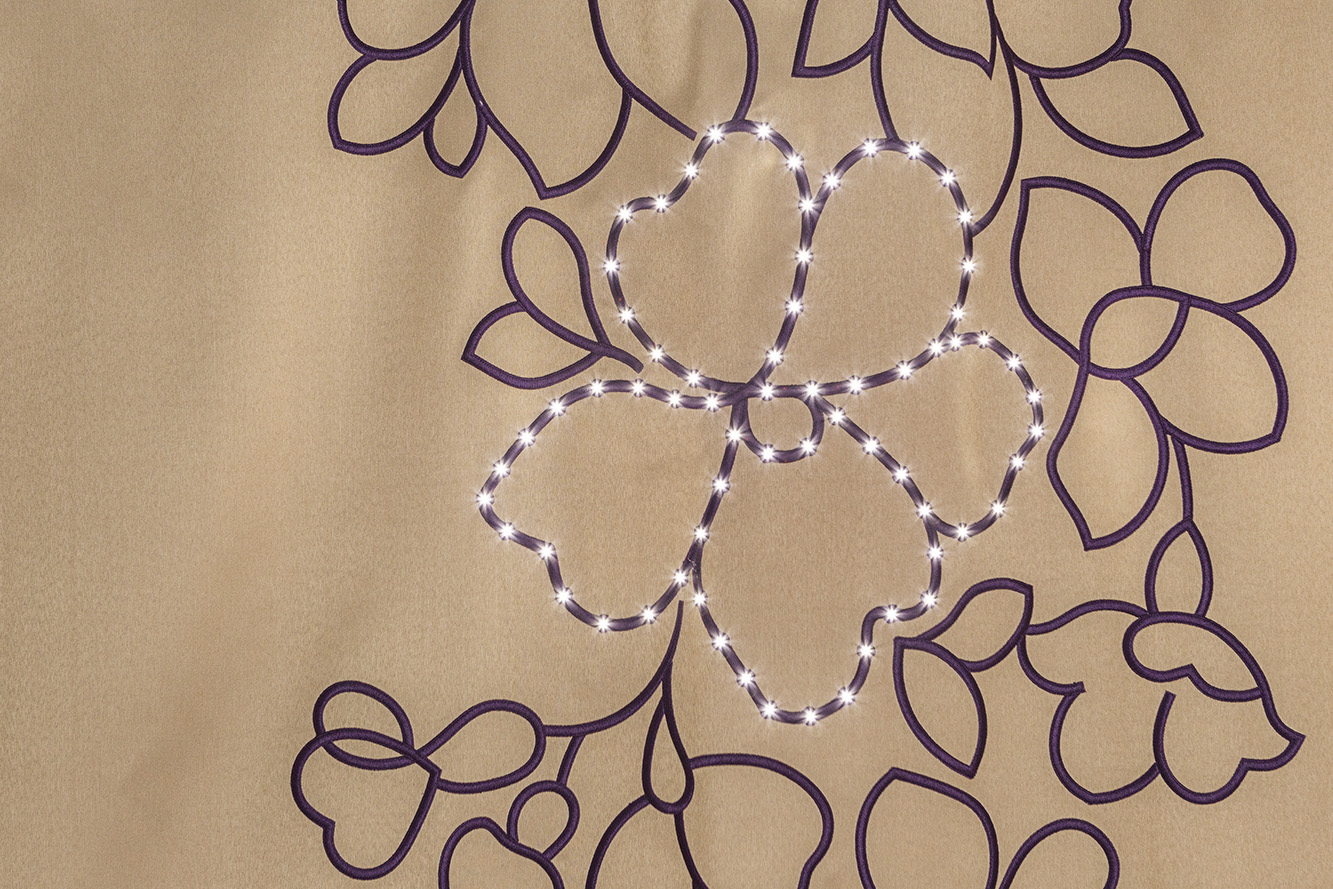
\includegraphics[width=10cm]{DIMOUT-MATT-BOUQUET_camel_WEB.jpg}
\caption{e-broidery制成的时装布料} 
\label{e2}
\end{figure}

http://www.frti.ch/en/

http://www.e-broidery.ch/en/





\chapter{技术方案及具体实现}

本章着重叙述我们选取的技术方案及具体实现的探索过程,从元件选型到最终的整体整合。如下:

\begin{itemize}
\item 元件选型
\item 工艺探索
\item  整体整合
\end{itemize}

\section{元件选型}


\subsection{WS2812(LilyPad Pixel)}

WS2812B是一个集控制电路与发光电路于一体的智能外控LED光源。其外型与一个5050LED灯珠相同,每个元件即为一个像素点。像素点内部包含了智能数字接口数据锁存信号整形放大驱动电路,还包含有高精度的内部振荡器和可编程定电流控制部分,有效保证了像素点光的颜色高度一致。数据协议采用单线归零码的通讯方式,像素点在上电复位以后,DIN端接受从控制器传输过来的数据,首先送过来的24bit数据被第一个像素点提取后,送到像素点内部的数据锁存器,剩余的数据经过内部整形处理电路整形放大后通过DO端口开始转发输出给下一个级联的像素点,每经过一个像素点的传输,信号减少24bit。像素点采用自动整形转发技术,使得该像素点的级联个数不受信号传送的限制,仅仅受限信号传输速度要求。LED具有低电压驱动,环保节能,亮度高,散射角度大,一致性好,超低功率,超长寿命等优点。将控制电路集成于LED上面,电路变得更加简单,体积小,安装更加简便。

传统方式要控制多颗RGB LED在电路接线和程式控制方面是非常烦杂的,然而使用内建WS2812晶片的RGB LED却是简单又方便,不管你要控制几颗RGB LED,都只要使用Arduino 3支脚位就足够了。


\begin{figure}[htbp]
\centering
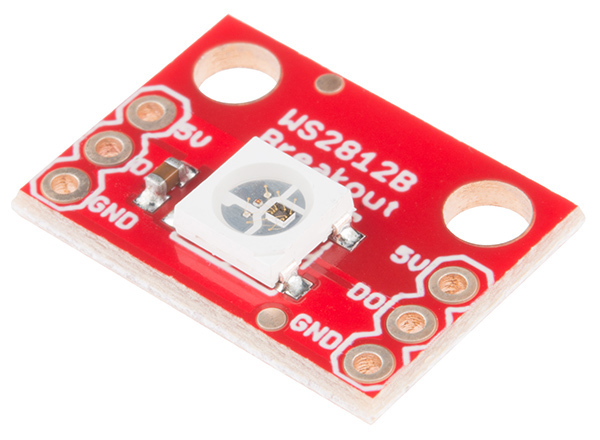
\includegraphics[width=10cm]{WS2812B.jpg}
\caption{WS2812 Breakout板} 
\label{2812}
\end{figure}

相比于WS2812 Breakout板,LilyPad Pixel 的LED则是位于一个紫色的圆环之内。这种做法使它有利于缝合在衣物或者其他纺织物,那么就可以很方便的嵌入我们的智能纺织物的项目中。

\begin{figure}[htbp]
\centering
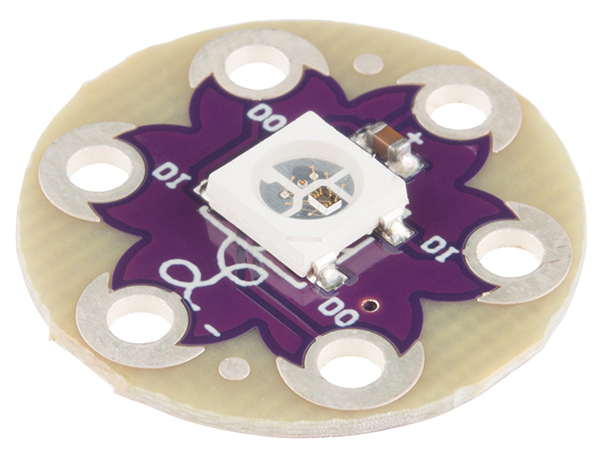
\includegraphics[width=10cm]{Lilypad_Pixel.jpg}
\caption{LilyPad Pixel} 
\label{LilyPad}
\end{figure}

% http://www.i-element.org/ws2812/


WS2812比乍一看以为的复杂的多,它看起来像一个普通的5050-sized(5x5mm)LED,但实际上远不止这么简单,它里面是有一个电流控制集成电路的。如果你仔细看的话,你会看到那些藏在里面的微小的芯片, 芯片上还有几根金丝连接到LED上。

\begin{figure}[htbp]
\centering
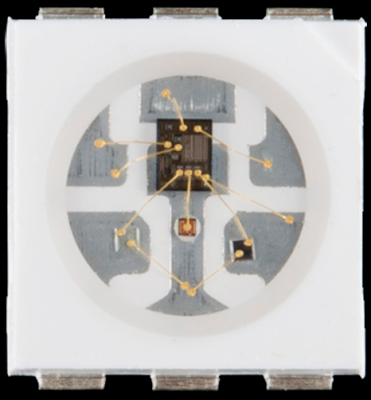
\includegraphics[width=10cm]{51f02cd5ce395fdb0f000001.png}
\caption{WS2812的内部细节} 
\label{WS}
\end{figure}

这款LED本身很像普通的RGB(红、绿、黄)LED。每一种颜色的亮度可以通过脉宽调制,,,实现256级的分级控制。这意味着它能通过组合RGB的亮度,实现16,777,216(2563)种颜色。所以你可以调制出任何的颜色,无论是白色到黑色(关闭RGB),还是到橙色到红褐色。
\begin{figure}[htbp]
\centering
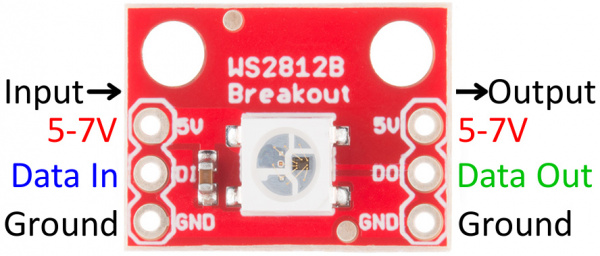
\includegraphics[width=10cm]{Ws2812B_Pins.jpg}
\caption{WS2812电路板的引出脚} 
\label{WSq}
\end{figure}

这款电路板安置有一颗多彩LED在板上,并且留出了几个引脚用于控制LED。

下面我们来介绍一下四个独立的引脚:

5V-这个引脚需要由一个5V-7V的直流电源接入。电压过高(7V)的话会烧毁LED,电压太低(5V)的话则会造成亮度过低,甚至造成LED不工作。

GND-公共引脚,接地,即接电源的负极。

DI-微控制器(或者是另外一个WS2812)的数据从这个引脚传入LED。

DO-数据从这里输出给下一级的WS2812,如果这个WS2812是最后一级,则可直接悬空此引脚。

数据传输接口

这个用于微处理器和WS2812数据传输的接口只有一条线,但是却不像已有的标准,如UART串行接口。这个接口的时序很特别。只有逻辑0和逻辑1,而逻辑0或1各有它们自己对应的脉冲宽度。

\begin{figure}[htbp]
\centering
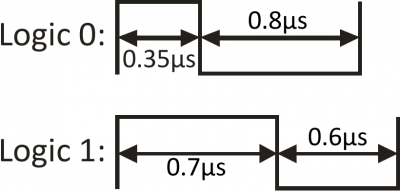
\includegraphics[width=10cm]{51f04d33ce395f687c000001.png}
\caption{逻辑0和逻辑1的时序图} 
\label{WS01}
\end{figure}

在一个低电平的复位脉冲(至少维持50us)后,这些数据以24位二进制数–每种颜色8位二进制数,被按顺序地发送出去.

一串24位二进制数–每种颜色8位二进制数。先是绿色,然后是红色,最后是蓝色。

某种特定的颜色(RGB之一)的值越大,则这种颜色的亮度越大。如果每种颜色(RGB)都被设置为0,则LED被关闭。如果每种颜色都被设置为最大,即255,那么LED会显示为它能显示的最亮的白色。

综上所述,这个接口的时序是非常的特别的。为了让这些灯亮起来,需要一个能发出精确时间脉冲的处理器,例如Arduino或STM32;而树莓派或者pcDuino是不能发出精确时间脉冲的。如果有一位数据的脉冲周期短于1ms,则可能会造成LED发出深紫色的光而不是你要的纯紫色。

这种LED最棒的地方就在于它们很容易连在一起。微控制器的的一个引脚就可以控制起整个灯带。

组装电路的第一步就是要实现控制板和LED的可靠连接。需要把LilyPad Pixel板用电线缝起来,并用线把LED串起来,连成一条灯带。

通过连接DI和DO将WS2812板连成链状(供电)。

WS2812需要大约5V才能工作。它可以在4V到7V的范围内工作,但是5V的电源可以直接在很多的板子上引用过来。例如Arduino上的5V电源,就是一个很好的LED电源。

同时,我们也要考虑到灯带需要多少的电流去驱动。一般来说,一个亮度全开的LED,他的板子需要至少60mA(每个通道20mA)。如果把10块LED板连到一起,那么你最好找一个600mA的电源。如果串了很多个这些LED,那就要确保电源能提供上这些电流。如果你最后决定你要用一个外部电源,那你要确保你的电源地和Arduino的地有连到一起。我们使用的是12V的3S10C航模锂电,可以满足要求。

在WS2812连接电源前,在电源和地之间并联一个大电容。它的容值在100uF到1000uF间最好。

这个电容可以让你的电源输出更加平滑。WS2812的负载电流的变化范围很广,当电流上下变化时,它可以补偿电源的电流变化,保证电源的稳定输出。这个电容的作用相当于一个电源储备库,在电源充足的时候把能量储存起来。

在Arduino的输出口和WS2812的输入口间串联一个小电阻将会有助于保护输出口。阻值在220到470欧比较合适。最终选取的是470欧

\begin{figure}[htbp]
\centering
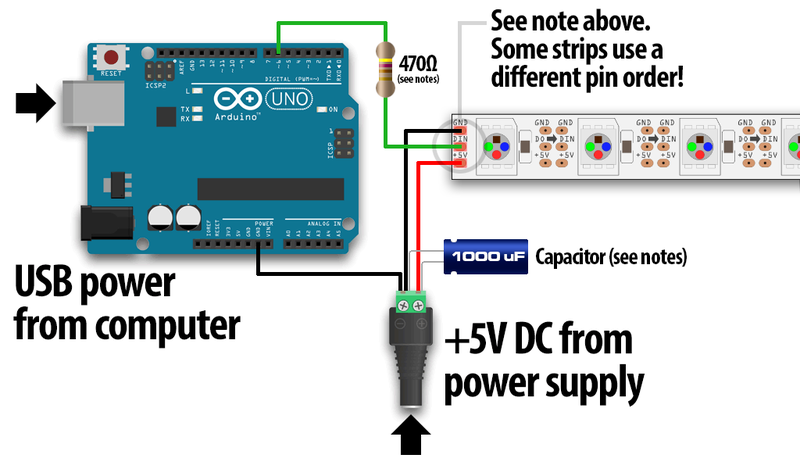
\includegraphics[width=10cm]{leds_Wiring-Diagram.png}
\caption{接线图} 
\label{WS012}
\end{figure}


\subsection{FLORA}

FLORA是Adafruit针对可穿戴设备推出的一款小型化开发平台,可以通过USB接口连接电脑,便于直接编程,同时它还支持USB HID。FLORA其实并不是第一个针对可穿戴设备的Arduino开发平台,Leah Buechley在2007年就设计制作过一款LilyPad,不过FLORA的闪存和SRAM是LilyPad的两倍,而且FLORA比LilyPad更小巧。

FLORA是织物友好的 - 板上的所有组件都与PCB齐平,不会阻碍精致的服装(它不使用FTDI接头)(FLORA is fabric friendly-- all the components on board are flush to the PCB and won't snag delicate garments (it does not use FTDI headers).),这也是我们选用FLORA的重要原因。

\begin{figure}[htbp]
\centering
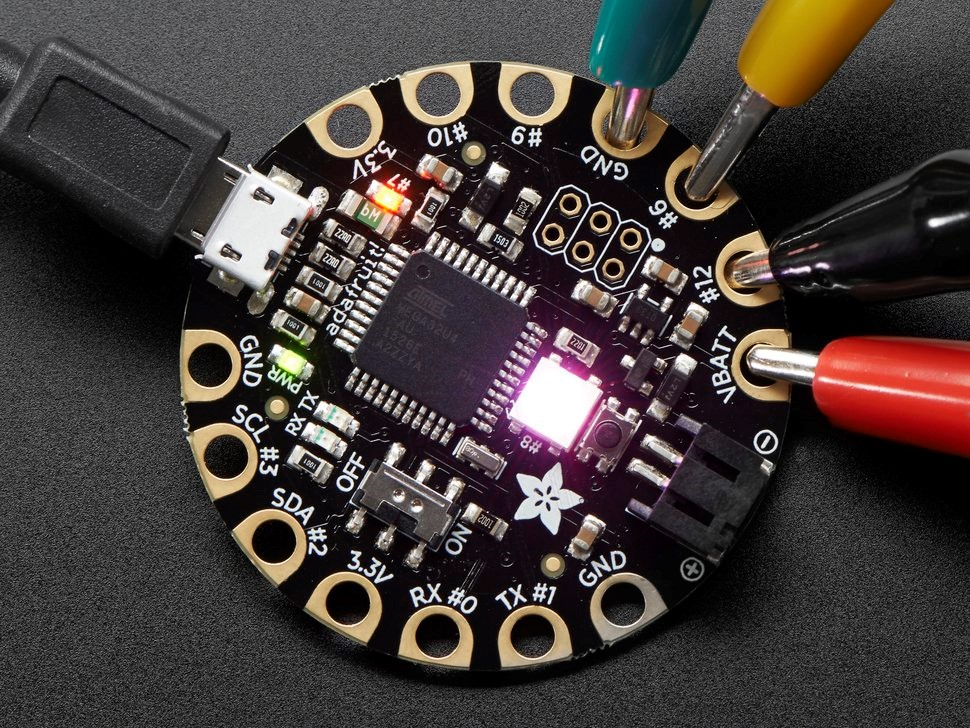
\includegraphics[width=10cm]{FLORA.jpg}
\caption{FLORA开发板} 
\label{FLORA}
\end{figure}

代码如下:

\begin{minted}{c}

#include <Adafruit_NeoPixel.h>

#define PIN 8

Adafruit_NeoPixel strip = Adafruit_NeoPixel(1, PIN, NEO_GRB + NEO_KHZ800);

void setup() {
  strip.begin();
  strip.setBrightness(50);
  strip.show(); // Initialize all pixels to 'off'
}

void loop() {
  // Some example procedures showing how to display to the pixels:
  colorWipe(strip.Color(255, 0, 0), 500); // Red
  colorWipe(strip.Color(0, 255, 0), 500); // Green
  colorWipe(strip.Color(0, 0, 255), 500); // Blue
  rainbowCycle(20);
}

// Fill the dots one after the other with a color
void colorWipe(uint32_t c, uint8_t wait) {
  for(uint16_t i=0; i<strip.numPixels(); i++) {
      strip.setPixelColor(i, c);
      strip.show();
      delay(wait);
  }
}

// Slightly different, this makes the rainbow equally distributed throughout
void rainbowCycle(uint8_t wait) {
  uint16_t i, j;

  for(j=0; j<256*5; j++) { // 5 cycles of all colors on wheel
    for(i=0; i< strip.numPixels(); i++) {
      strip.setPixelColor(i, Wheel(((i * 256 / strip.numPixels()) + j) & 255));
    }
    strip.show();
    delay(wait);
  }
}

// Input a value 0 to 255 to get a color value.
// The colours are a transition r - g - b - back to r.
uint32_t Wheel(byte WheelPos) {
  WheelPos = 255 - WheelPos;
  if(WheelPos < 85) {
   return strip.Color(255 - WheelPos * 3, 0, WheelPos * 3);
  } else if(WheelPos < 170) {
    WheelPos -= 85;
   return strip.Color(0, WheelPos * 3, 255 - WheelPos * 3);
  } else {
   WheelPos -= 170;
   return strip.Color(WheelPos * 3, 255 - WheelPos * 3, 0);
  }
}
\end{minted}
% https://learn.adafruit.com/getting-started-with-flora/blink-onboard-neopixel


\subsection{TGAM脑电模块}
TGAM模块包括了TGAT芯片,该芯片是一个高度集成的单一芯片脑电传感器,可以输出三个Neurosky的eSense参数,可以进行模数转换,检测接触不良的异常状态,过滤掉眼电噪音及50/60hz交流电干扰。

此TGAM模块可以处理并输出脑波频率谱,脑电信号质量,原始脑电波和三个Neurosky的eSense参数:专注度,放松度和眨眼侦测。和人体的界面只需一个简单的干接触点,所以可以很容易的运用于玩具,视频游戏和健康设备中,又由于能耗小,适合用在以电池供电的便携式消费产品的应用上。

\begin{figure}[htbp]
\centering
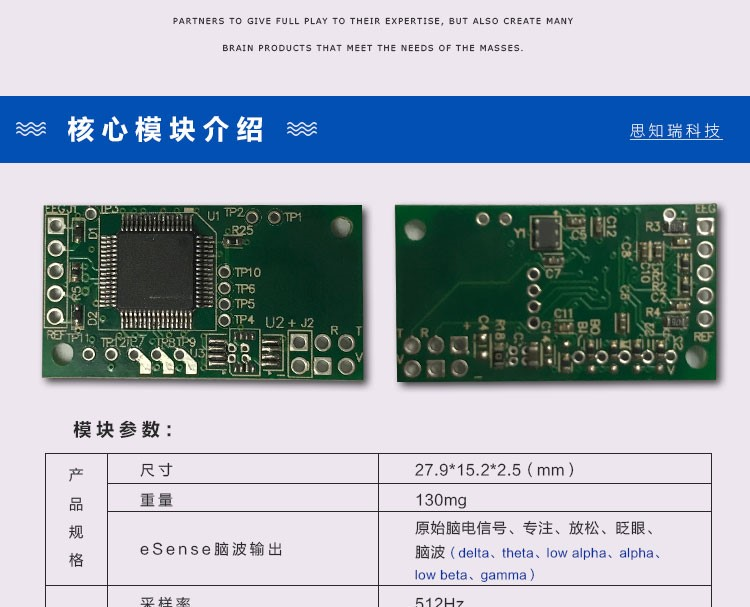
\includegraphics[width=10cm]{TGAM.jpg}
\caption{TGAM模块} 
\label{TGAM}
\end{figure}

http://www.neurosky.com.cn/products-markets/eeg-biosensors/hardware/

用TM4C123GH6PM解析TGAM数据包

本次开发使用神念科技的TGAM模块,该模块突破了医用常规的湿传感器使用上的不便,TGAM和人体的接触只需要一个简单的干接触点,使用时,用一电极夹住左耳垂作为基准电位,另一电极放置左前额进行测量。

开发过程较为困难,因为刚开始一无所知,正应了一句话万事开头难。脑电模块是同学借给我们的,但并没有提供任何资料,仅知道需要蓝牙连接,接收数据。最开始的摸索,甚至连电源开关都没找到,后来更替了新电池,按下一个隐蔽的小按钮,发现有指示灯亮起,估计是可以工作了。

之后就是查阅先关资料,第一个咨询对象就是淘宝,主要是找淘宝上类似产品,通过图示了解使用方法。淘宝在这次开发中的确提供了我很大帮助,之后还会具体提到。淘宝上同类型产品价值都在数百元以上,可见该类产品的确属于高端产品。另一个队员向用过该模块的学长求助,学长只提供了一份TGAM数据了格式说明书,后来我也在网上找到了这份说明,所以这位学长的帮助不占主要地位。真正的突破还是神念科技的官网,不过链接倒是通过那份说明书找到了。官网上有一些产品和应用的介绍,还提供了各种资料的下载,例如APP和供再开发的SDK。后来仔细研究了从中下载的资料,发现有PC端开发程序以及其他平台(包括微控制器)开发使用的API。

首先肯定要在PC端实现基本的数据解析功能,根据相关说明书的指导,需要将脑电波模块的蓝牙与PC连接,然后运行解析程序(C语言版本),不过需要配置蓝牙连接所在的COM口。连接成功后,成功运行C程序,得到解析的数据。我们使用realterm来观察脑电波模块数据包,不过在我们开发过程中,这款软件仅用来测试是否接收到了数据。

\begin{figure}[htbp]
\centering
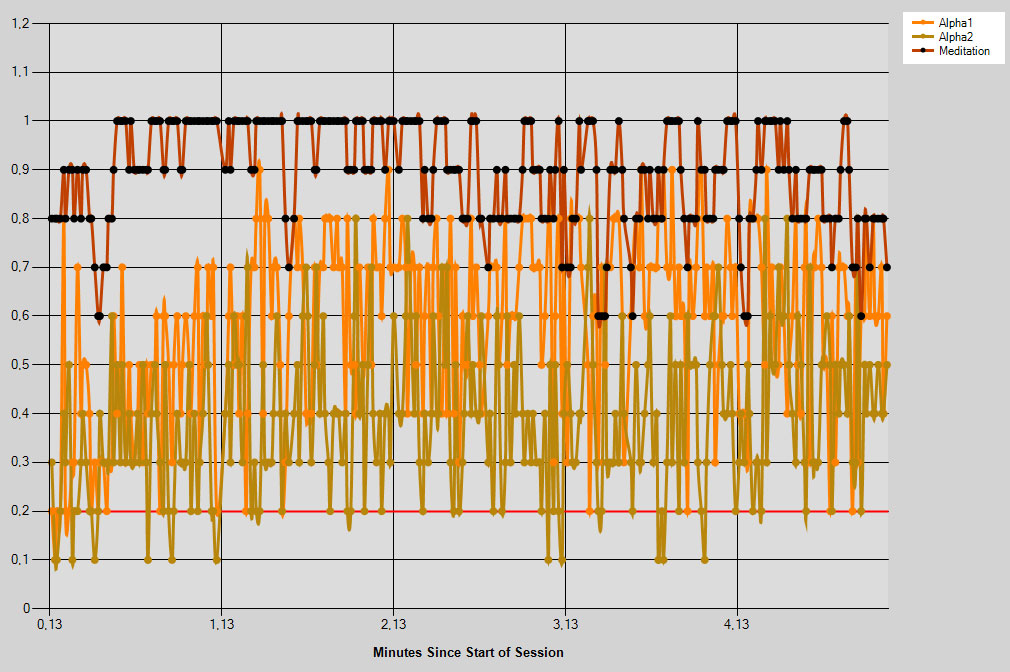
\includegraphics[width=10cm]{neuroexperimenter14.jpg}
\caption{realterm解析出的数据绘制的图表} 
\label{realterm}
\end{figure}

PC端解析的成功,鼓舞我将其移植到微控制器上。基本思路还是有的,首先要配置微控制器UART模块,然后在硬件上与一个蓝牙模块连接,之后想办法让微控制器上的蓝牙与脑电波模块上的蓝牙配对。最后配对的过程需要通过微控制器发送AT指令的形式实现蓝牙模块间的配对。

配对上,首先两个模块要一主一从,由于脑电波模块可以被搜索到和配对,可以相信它是从模式,我们自己的模块就要为主模式,然后主模式搜索找到附近可以配对的蓝牙地址,进而配对,检查对方模块是否在配对列表中,下次使用直接连接即可。不过期间也有个问题,进入AT模式有两种方法,一是电源和EN同时上电拉高,不过此时使用固定波特率38400,而我们的脑电波模块波特率为57600,此时配对后也难以改变波特率,所以数据包不可能正确解析出来,二是先上电再拉到EN,此时为模块自身设定好的波特率,如果我们事先将其波特率设为57600,那么配对连接好仍可以使用这个波特率接收数据解析数据。

配对成功后,开始研究如何把UART接收的数据用以解析,我找到了先关API函数(一个.c和一个.h文件)。我把例程移植到微控制器代码上,需要修改的就是数据读取方式,源代码是C语言使用文件相关的函数如fopen、fread等,它每次一个读取一个字节,既然如此就很容易将这一过程修改为UART每次读取一个字节,这是最主要的修改,此外还有其他一些细节修改不再赘述。

最后,说一下目前实现的效果和作品体验,目前可以在微控制器上解析出脑电波数据包,得到我们脑部活动的专注度和冥想度,大概一秒钟更新一次(受限于脑电波模块数据发送情况),然后显示在终端上。有些延迟,尤其在刚带上脑电波采集器时,需要数秒才会显示数值。摘下后,反应还可以,一两秒数值会变为0表示没有脑电数据。

目前这一套也成功的使用FLOAR跑通了。

读取UART脑电数据代码
\begin{minted}{c}
/*
 通过UART串口显示信号值、注意力及放松度的值
 */
#define BAUDRATE 57600
#define DEBUGOUTPUT 0

//校验相关变量
int   generatedChecksum = 0;
byte  checksum = 0; 

//接收数据长度和数据数组
byte  payloadLength = 0;
byte  payloadData[32] = {0};//总共接收32个自己的数据

//需要读取的信息变量
byte signalquality = 0;//信号质量
byte attention = 0;    //注意力值
byte meditation = 0;   //放松度值

//初始化
void setup() 
{
  Serial.begin(BAUDRATE); 
}

//从串口读取一个字节数据
byte ReadOneByte() 
{
  int ByteRead;
  while(!Serial.available());
  ByteRead = Serial.read();
  return ByteRead;//返回读到的字节
}

//读取串口数据
void read_serial_data()
{
    //寻找数据包起始同步字节,2个
    if(ReadOneByte() == 0xAA)//先读一个
    {
      if(ReadOneByte() == 0xAA)//读第二个
      {
        payloadLength = ReadOneByte();//读取第三个,数据包字节的长度
        if(payloadLength == 0x20)//如果接收到的是大包数据才继续读取,小包数据则舍弃不读取
        {
          generatedChecksum = 0; //校验变量清0       
          for(int i = 0; i < payloadLength; i++)//连续读取32个字节
          {  
            payloadData[i] = ReadOneByte();//读取指定长度数据包中的数据
            generatedChecksum += payloadData[i];//计算数据累加和
          }         
          checksum = ReadOneByte();//读取校验字节  
          //校验
          generatedChecksum = (~generatedChecksum)&0xff;       
          //比较校验字节
          if(checksum == generatedChecksum)//数据接收正确,继续处理 
          {    
            signalquality = 0;//信号质量变量
            attention = 0;    //注意力值变量
            //赋值数据
            signalquality = payloadData[1];//信号值      
            attention = payloadData[29];//注意力值
            meditation = payloadData[31];//放松度值
            #if !DEBUGOUTPUT         
            //打印信号质量
            Serial.print("SignalQuality: ");
            Serial.print(signalquality, DEC);
            //打印注意力值
            Serial.print("Attation: ");
            Serial.print(attention, DEC);
            //打印放松度值
            Serial.print("Meditation: ");
            Serial.print(meditation, DEC);
            //换行
            Serial.print("\n");       
            #endif              
          } 
        } 
      }
    }
}

//主循环
void loop() 
{
  read_serial_data();//读取串口数据 
}

\end{minted}
%include 不能嵌套

%https://blog.csdn.net/qq_27163279/article/details/78430651

\section{工艺探索}


\subsection{线材}
直接选用0.04mm直径的直焊型 QA-1-130 漆包线,室温电阻小于10欧/米,可弯曲性很好,且表面有绝缘层,可防止编织时两线交叉而造成的短路,机械强度和拉伸系数也完全符合项目要求。

\begin{figure}[htbp]
\centering
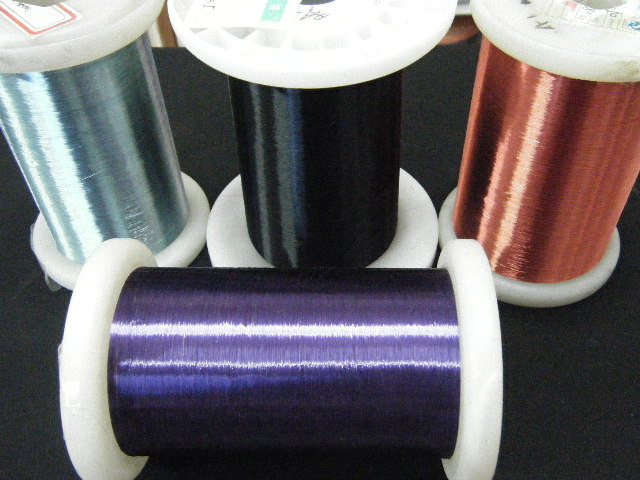
\includegraphics[width=10cm]{T2C.jpg}
\caption{直焊型 QA-1-130 飞线} 
\label{r}
\end{figure}

后期可能改用先进一些的新材料,比如导电织物专用的线材:https://patents.google.com/patent/CN104674573A/zh 。

%https://detail.tmall.com/item.htm?id=568698277535&ali_refid=a3_430582_1006:1123935064:N:%E6%BC%86%E5%8C%85%E7%BA%BF%20%E9%93%9C%E7%BA%BF:4ff942c403e010968b28f5aeb937b2c4&ali_trackid=1_4ff942c403e010968b28f5aeb937b2c4&spm=a230r.1.14.1

\subsection{焊盘}

元件采用类似FLORA和LilyPad Pixel的织物友好的焊盘:宽大而且与元件平面齐平的焊盘。这样在保证柔性(有利于缝合在衣物或者其他纺织物)的同时,也增大了鲁棒性。(焊盘与导线接触面积大)

分线板则采用类似多旋翼集线板/电调分线板/植保无人机分电板的板式PCB,由于在整个电路中这种分线板只有一到两处,而且板面极小,不会影响织物的穿戴整体体验。

\begin{figure}[htbp]
\centering
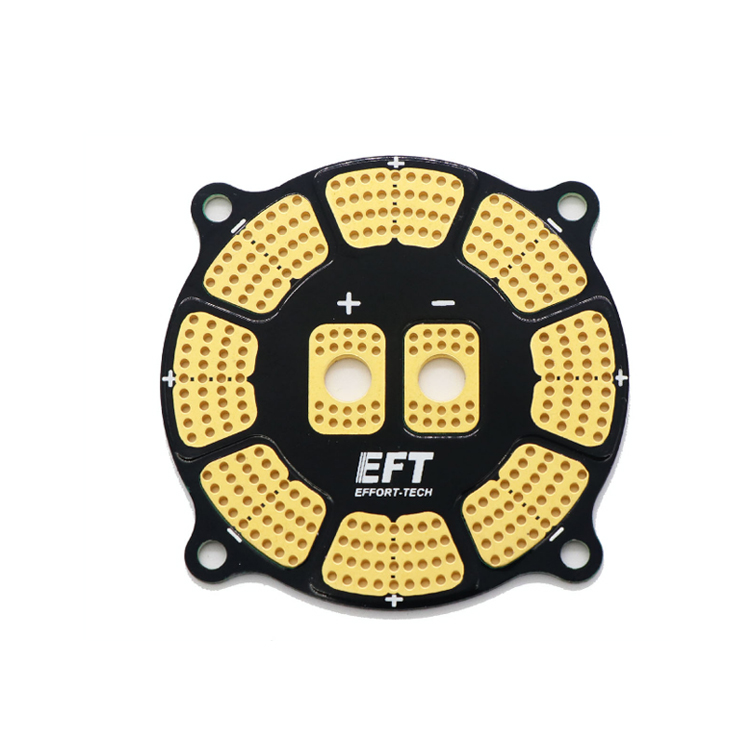
\includegraphics[width=10cm]{O1.jpg}
\caption{集线板/分线板} 
\label{r1}
\end{figure}

\subsection{整体电路与布料/衣物的整合}

首先讨论走线:由于对于电路鲁棒性的要求,我们将极细的一回漆包线(类似于双绞线)用缝纫机缝制到布料之中,由于大量使用的WS2813在项目中用到的是两进两出的串联结构,所以为了布线方便,两两连线均采用类似双绞线的缝制工艺。个别需要三线/四线并行的(如VCC和GND引线)使用四色缝纫机实现。如果无法避免出现单根导线情况,则使用两根等效的漆包线代替单根导线连接。

\begin{figure}[htbp]
\centering
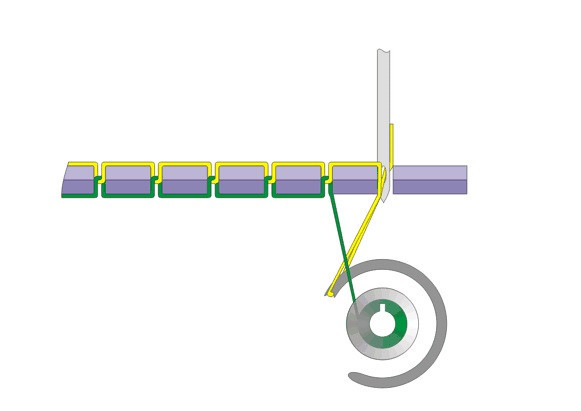
\includegraphics[width=10cm]{spfw04.jpg}
\caption{缝纫机缝制工艺示意图} 
\label{f1}
\end{figure}


其次对于LilyPad Pixel安置分单层薄纱和双层半透布料讨论:

\begin{itemize}
\item 对于双层半透布料,我们将LilyPad Pixel安放在两层布料之间,这样在日常生活和洗衣机机洗的时候能最大限度的保护焊盘连接处。
\item 单层薄纱则不同,我们将LilyPad Pixel放置在布料的一侧,使用时有LilyPad Pixel的一侧为外侧,由于四根“编织”漆包线的固定作用,日常使用不会脱落,但是使用洗衣机清洗则要慎重。
\end{itemize}

在批量生产时,可以定制纺织机实现高可靠性的自动生产,本作品仅展示这种缝制工艺的可行性。


\section{整体整合}

我们将上述电路连接并调试完成,目前正在进行将电路向织物内整合的工作。



\chapter{展望}
未来智能可穿戴设备的普遍应用,将促进柔性嵌入式电路的发展,本文提出的柔性电路工艺实现后将在不久的未来显示出其价值所在。

%\subsection{}